\documentclass{ituthesis}
\usepackage[]{hyperref}
\usepackage[]{float} 
\usepackage[]{csquotes} 
\usepackage[]{graphicx} 
\usepackage[]{caption} 
\usepackage[]{subcaption} 
\usepackage[]{natbib}
\bibliographystyle{agsm}

\settitle{The Practical Guide to Levitation}
\setauthor{Ahmad Salim Al-Sibahi}
\setsupervisor{Dr. Peter Sestoft}
\setextrasupervisor{David R. Christiansen}
\setdate{September 1, 2014}

\begin{document}
%\selectlanguage{danish}

\frontmatter

\thetitlepage
\newpage

\chapter*{Abstract}
Goal: Implementation of levitation in a realistic setting, with practical performance benefits.
\blockquote{DISCLAIMER: This is a draft and as such is incomplete, incorrect and can contain grammatical errors.
Although I claim originality of this report, many underlying ideas are based on current work in the scientific community which will be correctly attributed
when the work is complete.}

\cleardoublepage
\setcounter{tocdepth}{1}
\tableofcontents

\mainmatter

%from memoir documentation:
%TeX tries very hard to keep text lines justified while keeping the interword spacing as constant as possible, but sometimes fails and complains about an overfull hbox.
%The default mode for LaTeX typesetting is \fussy where the (variation of) interword spacing in justified text is kept to a minimum. Following the \sloppy declaration there may be a much looser setting of justified text.
%Additionally the class provides the \midsloppy declaration which allows a setting somewhere between \fussy and \sloppy.
%fewer overfull lines than \fussy, and fewer obvious large interword spacing than with \sloppy.
%the memoir manual also uses \midsloppy!
\midsloppy
% try harder to avoid widows and orphans
\sloppybottom

\chapter{Introduction}
\label{cha:Intoduction}
\section{Context}
\label{sec:Context}
Algebraic datatypes such as booleans, lists or trees form a core part of modern functional programming.
Most functions written work directly on such datatypes, but sometimes the function we write aren't directly dependent on the datatype itself and serve only as a repetitive exercise such as for structural equality or pretty printing.
In fact it seems that it is possible to write an algorithm over the structural definition of the datatype, which the computer then could use to derive an actual function for particular datatypes.

Enter the world of \textit{generic programming} where the target datatype is the one describing the structure of other datatypes, often called the \textit{description}.
While generic programming sounds promising, there has traditionally been issues regarding usability in ordinary functional languages such as Haskell. To represent the description, it is often required to use special language extensions and the programming style tend to be
orthogonal to writing ordinary programs.

However, in dependently-typed languages such as Idris or Agda it seems that it possible to mitigate such issues.
Due to the nature of dependently-typed languages it is possible to create a correct description using ordinary datatype definitions.
Furthermore, \cite{Chapman:2010:GAL:1863543.1863547} how it is possible to build a self-supporting type system which is able to synthesise descriptions to ordinary types while still being powerful enough to describe the description datatype itself.
Therefore in such system, generic programming is not different from ordinary programming in such system.

%\subsection{The Importance of Genericity in Dependently-typed Languages}
%\label{sub:TheImportanceofGenericityinDependently-typedLanguages}
%\textit{The similarity of structure and various slightly-different indexing of types.}


\section{Problem Definition}
\label{sec:ProblemDefinition}
The current work on generic programming in dependently-typed languages presents both elegant and correct ways to represent the structural descriptions of datatypes. Furthermore, it allows the programmer to save both time and boilerplate code by using ordinary techniques to do generic programming.

Yet in many ways, the state of the art is heavily theoretically oriented, which might lead to issues when a system needs to be developed with a practical audience in mind.
First of all, multiple incompatible descriptions are often presented in the current field, sometimes even in the same paper, which is not particularly attractive in a practical setting.
Secondly, there has been little work done on how to integrate such descriptions in languages which contain features such as type classes and proof scripts.
Finally, datatypes synthesised from descriptions create large canonical terms and as such both type checking and runtime performance is very slow.
In summary, if an efficient and easily usable framework for programming with described types that avoids the described issues could be implemented successfully, it would save programmers both the time and effort required when writing repetitive functions.

\section{Aim and Scope}
\label{sec:AimandScope}
The main aim of this research is to provide a practical and efficient implementation of described types in Idris.

One key part is to find a good definition of the description that supports many common datatypes.
I seek to mainly base my effort on reusing some of the existing work, and not try to improve underlying type theory to support more complex inductive families; neither will I focus on supporting all language features of Idris such as implicit arguments and codata definitions.
Another key part is to present realistic examples using generic functions by implementing functions that can be used to derive type class instances and a Scrap Your Boilerplate library for generic querying and traversal.
In the end, I seek to use partial evaluation to optimise the generic functions with regards to specific descriptions to try to achieve near hand-written performance metrics. %Elaborate when I know more about PE\ldots

\section{Significance}
\label{sec:Significance}
The main contributions of my research are:

\begin{itemize}
  \item an example-based tutorial for understanding described types in the context of a practical programming language, namely Idris
  \item an generic implementation of common operations such as decidable equality, pretty printing and functors, which can be used to provide default implementations to type class methods.
  \item a discussion of what challenges arise when trying to implement a SYB-style generics library in dependently typed languages
  \item optimisation techniques based on partial evaluation for reducing runtime size and time overhead for described types and accompanying generic functions
  \item metrics that show how generic programming using described types is a viable option to reduce boilerplate without significant cost in performance
\end{itemize}
\section{Overview}
\label{sec:Overview}
I will present the report as follows. In Chapter~\ref{cha:GenericProgramming}, I will present an introduction to described types specifically focusing on recent developments using dependently-typed programming languages.
In Chapter~\ref{cha:PartialEvaluation}, I will present an overview of techniques for partial evaluation of functions and specialisation of datatypes. In Chapter~\ref{cha:LevitatingIdris}, I will discuss specifically how described types are implemented in Idris and I will continue with the practical examples in Chapter~\ref{cha:PracticalExamples}.
In Chapter~\ref{cha:OptimizingIdrisforFlight} I will present what optimisations were made in order to improve the runtime performance of described types and generic functions. I will evaluate the results in Chapter~\ref{cha:Evaluation}, comparing the performance of generic implementations to hand-written ones.
Finally, I will discuss what challenges still lie ahead and conclude in Chapter~\ref{cha:Discussion}.
\chapter{Generic Programming}
\label{cha:GenericProgramming}
\section{The Generic Structure of Inductive Data Types}
\label{sec:TheGenericStructureofInductiveDataTypes}
\subsection{Anatomy of a Datatype}
\label{sub:AnatomyofaDatatype}
In order to understand how a description might look like, let us first start by looking closely at how datatypes are structured. In Figure~\ref{fig:anatomydatatype}, I will present an annotated version of a typical dependently-typed datatype representing vectors.

\begin{figure}[ht]
\begin{center}
    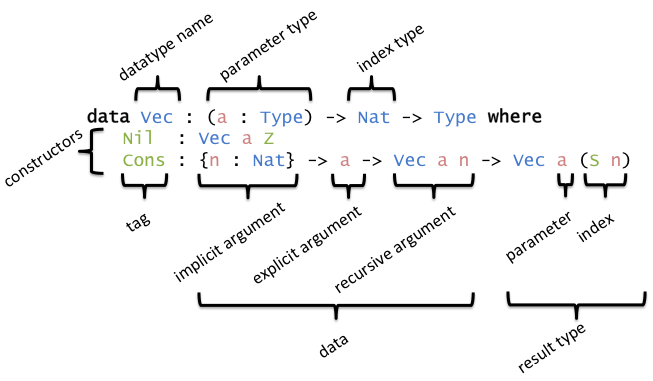
\includegraphics[scale=0.5]{Figures/AnatomyOfADatatype.png}
\end{center}
\caption{Annotated Components of a Datatype Declaration}
\label{fig:anatomydatatype}
\end{figure}

A datatype consists of a type constructor which describes what type-level arguments are required, and zero or more data constructors which describe how to create values of the datatype.
The type constructor consists of three components: a name for the datatype, types of any possible parameters, and the types of possible indices.
In Figure~\ref{fig:anatomydatatype} there is no difference between a parameter type or an index type since Idris figures that out automatically.\footnote{If the argument to a type constructor doesn't change in the data constructor declarations Idris considers that a parameter, and otherwise an index.}

Similarly to the type constructor, data constructors need names too, also called \textit{tags}.
Following the tag, the data constructor declaration contains the types of the arguments stored in the constructor and the resulting type which must use the type constructor of the datatype.
In our example two constructors are declared, \texttt{Nil} and \texttt{Cons}.
\texttt{Nil} doesn't hold any data, so it only needs to define the resulting type which is \texttt{Vect a Z} (a vector with length 0).
\texttt{Cons} contains three different types of arguments: an ordinary implicit argument, an ordinary explicit argument, and an explicit argument to the type itself (recursive); the resulting type for \texttt{Cons} is \texttt{Vect a (S n)} (i.e. a vector of length 1+n where n is the length of the recursive argument).

\subsection{A Description for Datatypes}
\label{sub:ADescriptionforDatatypes}
It is now possible to try to represent a suitable description datatype. Figure~\ref{fig:descriptiondatatype} presents one possible solution, influenced mainly by the work of \cite{mcbride2010ornamental} and \cite{diehl2014eliminators}.

\begin{figure}[ht]
\begin{center}
    \includegraphics[scale=0.5]{Figures/ADescriptionforDatatypes.png}
\end{center}
\caption{Datatype for describing other Datatypes}
\label{fig:descriptiondatatype}
\end{figure}

In order to allow datatypes to be indexed by values of various types, the description structure takes a parameter that describes what the type of indices must be.
Additionally, the description has three constructors:
\begin{itemize}
  \item  \texttt{Ret} represents the end of a description and takes as argument what value the index of the resulting type must be
  \item  \texttt{Arg} represents the addition of an argument of any type to a given description; the first argument of \texttt{Arg} is the type of argument expected and the second argument is the rest of the description dependent on a value of that type.
  \item  \texttt{Rec} represents a recursive argument of the described datatype and take two arguments: the index of the recursive instance of the datatype and the rest of the description.
\end{itemize}

\begin{figure}[ht]
\begin{center}
    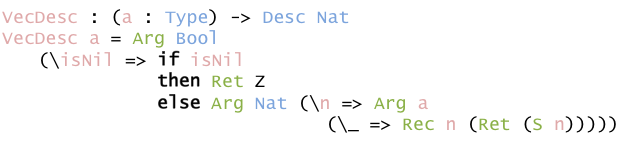
\includegraphics[scale=0.5]{Figures/VectorDescription.png}
\end{center}
\caption{Described version of Vec}
\label{fig:descvec}
\end{figure}

The astute reader might at this point have some questions such as: how is it possible to choose between different constructors? where do parameters go in the description? and why is there only one type for indicies?
I will now try to answer these questions using Figure~\ref{fig:descvec}.

One step towards building a value that describes a particular datatype is defining its type signature
including what types the parameters and indices of the finished datatype are. In our example of Figure~\ref{fig:descvec},
the parameter is specified to be given as an argument to the description value and is not represented internally as such in the final description, i.e., it is not possible to distinguish a parameter from other values when the final description is constructed.
Contrary to parameters, the type of indices must be specified as an internal part of the description in order to ensure that indices specified by recursive arguments match in the final description.
Since \texttt{Desc} only takes one argument for specifying the types of indices, more demanding datatypes will need to collect multiple indices into one dependent pair, e.g.,
a datatype with signature \texttt{(n : Nat) -> Fin n -> Type} must use the dependent pair \texttt{(n : Nat ** Fin n)} as the type for its index.

Another step required for describing a datatype is defining how to choose a particular constructor.
A solution could be the one presented in Figure~\ref{fig:descvec} where a boolean argument \texttt{isNil} is used to decide whether the resulting description should be for the \texttt{Nil} or \texttt{Cons} constructors.
However, since this solutions is fairly primitive and doesn't capture information such as constructor tags, a better but more complex encoding will be presented in Section~\ref{sub:AnInformativeEncodingofConstructors}.

Finally, the constructors themselves must be described.
\texttt{Nil} doesn't contain any data so we simply use \texttt{Ret Z} which indicates that the description is finished and the resulting type is expected to have index \texttt{Z}, analogously to Figure~\ref{fig:anatomydatatype}.
\texttt{Cons} takes first two ordinary arguments: a \texttt{Nat} argument\footnote{Implicit arguments is a feature of Idris that only works on top-level declarations and as such are all specified explicitly in the description.} to be used to describe the necessary indices, and an argument of the parameter \texttt{a}. Following these arguments we take a recursive argument---specified using \texttt{Rec}---that must satisfy to have the value of the input \texttt{Nat} argument \texttt{n} as index, i.e. the argument must be of type \texttt{Vect a n}. We finish the description with \texttt{Ret} and specify that the resulting index must be \texttt{S n} as expected.

\subsection{An Informative Encoding of Constructors}
\label{sub:AnInformativeEncodingofConstructors}
In Section~\ref{sub:ADescriptionforDatatypes} I had presented the choice of constructors using a boolean variable and concluded that it was both primitive and lacked
necessary information such as the tag of a particular constructor. I will in this section present a more informative encoding of constructors, and show how it is possible to use that encoding when describing datatypes.

In order to represent which constructors are available we first are going to declare two types as shown in Figure~\ref{fig:ctorlabels}: \texttt{CLabel} which represents a name for a constructor, and \texttt{CEnum} which
represents a list of constructor names. Figure~\ref{fig:vectctors} show an example of how to represent the available constructor names of \texttt{Vec}.


\begin{figure}[ht]
\begin{center}
  \subcaptionbox{Representation\label{fig:ctorlabels}}[.45\textwidth]{
    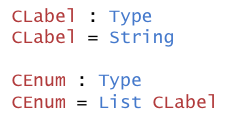
\includegraphics[scale=0.5]{Figures/AnInformativeEncodingofConstructorsLabels.png}
}
\subcaptionbox{Example: Constructors of Vec\label{fig:vectctors}}[.45\textwidth]{
    
\includegraphics[scale=0.5]{Figures/VectorConstructors.png}

}
\caption{Constructor Labels}
\end{center}
\end{figure}

Now that it is possible to represent the available constructors, we can encode a way of choosing a particular constructor tag. Figure~\ref{fig:ctortags} shows a datatype \texttt{Tag} with two constructors:
\texttt{TZ} which represents the constructor that is on top of the current list and \texttt{TS} which represents a constructor further along the list. As such, \texttt{Tag} specifies is valid index into a (non-empty) list of constructor tags.

\begin{figure}[ht]
\begin{center}
    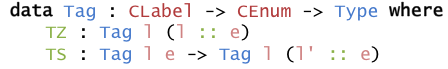
\includegraphics[scale=0.5]{Figures/AnInformativeEncodingofConstructorsTags.png}
\end{center}
\caption{Tags: A Structure for Picking a Constructor from a Label Collection}
\label{fig:ctortags}
\end{figure}

\subsection{A Constructive Type of Choice}
\label{sub:AConstructiveTypeofChoice}

Given a specific constructor tag, one question is then how it is possible to map these constructor tags to specific values? Figure~\ref{fig:smallpiop} presents $\pi$ (small pi operator) which represents
the type of a map from a list of constructor tags to a corresponding list of values.
The calculated type might look atypical at first, however on a closer look it is actually analogous to how lists are represented in Lisp.
The calculated type consists of nested pair types where the first element is the type of the value mapped for the current constructor
and the second element is the mapping for the rest of the constructors; finally, the list ends with the unit type \texttt{()} similarly to \texttt{nil} in Lisp.

\begin{figure}[ht]
\begin{center}
    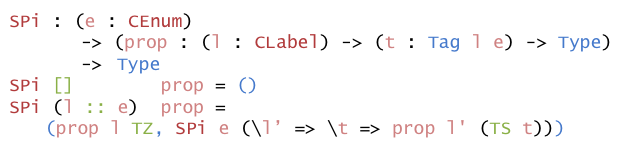
\includegraphics[scale=0.5]{Figures/AConstructiveTypeofChoice.png}
\end{center}
\caption{The Small Pi Operator: Type for Case Analysis based on Constructor Tags}
\label{fig:smallpiop}
\end{figure}

The \texttt{switch} function shown in Figure~\ref{fig:switchctor} uses a specific constructor tag to lookup the corresponding value given by the $\pi$ mapping.
When the given $\pi$ mapping is given inline switch works like a version of the \texttt{case of} operator on constructor tags, which can be useful when specifying descriptions for a particular constructor.

\begin{figure}[ht]
\begin{center}
    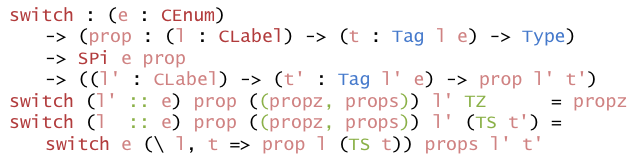
\includegraphics[scale=0.5]{Figures/AConstructiveChoice.png}
\end{center}
\caption{Calculation of a Property based on a Specific Constructor Tag}
\label{fig:switchctor}
\end{figure}

As an example, Figure~\ref{fig:vecdescim} shows the description of \texttt{Vec} again, but this time using the new constructor tag encoding instead of a boolean variable.
While the description might initially seem more complicated than before, it has a couple of clear advantages: the encoding now contain the constructor tag and it is possible to choose between more than two constructors at the same time.

\begin{figure}[H]
\begin{center}
    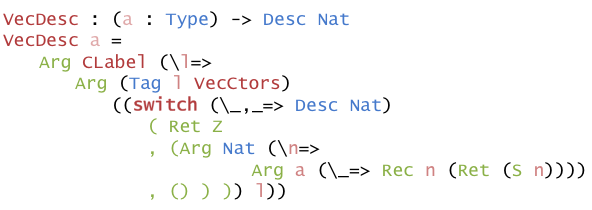
\includegraphics[scale=0.5]{Figures/VectorDescriptionImproved.png}
\end{center}
\caption{Description of Vec given a Constructor Tag}
\label{fig:vecdescim}
\end{figure}

%\subsection{Advanced Example: Representing a Finger Tree}
%\label{sub:Advanced Example:RepresentingaFingerTree}


%\begin{figure}[ht]
%\begin{center}
    %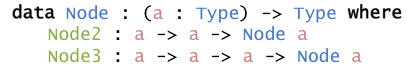
\includegraphics[scale=0.5]{Figures/AdvancedExampleNodeData.png}
%\end{center}
%\caption{Test}
%\label{fig:exnodedata}
%\end{figure}

%\begin{figure}[ht]
%\begin{center}
    %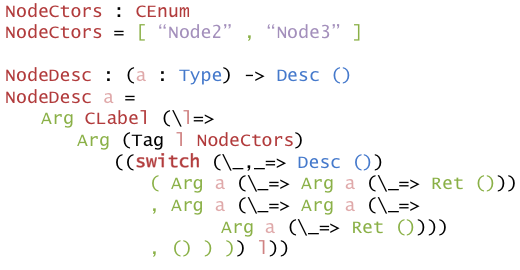
\includegraphics[scale=0.5]{Figures/AdvancedExampleNodeDescription.png}
%\end{center}
%\caption{}
%\label{fig:exnodedesc}
%\end{figure}

%\begin{figure}[ht]
%\begin{center}
    %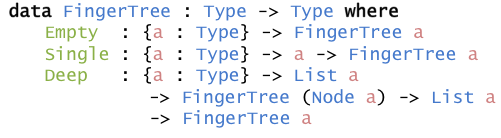
\includegraphics[scale=0.5]{Figures/AdvancedExampleFingerTreeData.png}
%\end{center}
%\caption{Test}
%\label{fig:exftdata}
%\end{figure}

%\begin{figure}[ht]
%\begin{center}
    %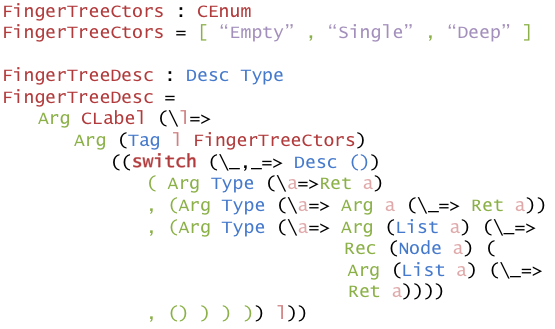
\includegraphics[scale=0.5]{Figures/AdvancedExampleFingerTreeDescription.png}
%\end{center}
%\caption{}
%\label{fig:exftdesc}
%\end{figure}



\section{Synthesising Descriptions to Types}
\label{sec:SynthesisingDescriptionstoTypes}
In Section~\ref{sec:TheGenericStructureofInductiveDataTypes} I had shown how it was possible to create descriptions that support many common datatypes in Idris.
In this section I will present a way to convert or \textit{synthesise} these descriptions to actual types in Idris, that allows the programmer to construct values of these described types with actual data.

\subsection{A Heterogeneous Form of Equality}
\label{sub:AHeterogeneousFormofEquality}
Before we proceed with the actual synthesis I would like to present one of the important types that is needed.
The type is called heterogeneous equality and is built into the core language theory of Idris.
\begin{figure}[ht]
\begin{center}
    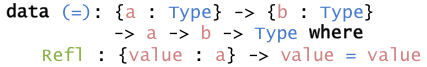
\includegraphics[scale=0.5]{Figures/HeterogeneousEquality.png}
\end{center}
\caption{Heterogeneous Equality of Values}
\label{fig:heteq}
\end{figure}
What the heterogeneous equality type allows us to do is that it allows us to construct a type that equate values of different types.
However in order to actually construct a value of such type (i.e., provide a proof for the equality), we have to use \texttt{Refl} which will only succeed if the compiler believes that such two values are really the same.
This provides a simple yet powerful way to constrain values in order to ensure that any given input must conform to some expected form.

\subsection{Datatype Synthesis}
\label{sub:DatatypeSynthesis}
It is finally time to convert the description to an actual type. Figure~\ref{fig:synthdata} shows the \texttt{Synthesise} method which takes a description, the final form of that datatype and the resulting index, then it returns a type which can contain the described data.

\begin{itemize}
  \item If we reach the end of the description, i.e. \texttt{Ret}, the only thing that we need to ensure is that the provided resulting index matches the expected index provided in the description. In order to apply such constraint we use the heterogeneous equality type (see Section~\ref{sub:AHeterogeneousFormofEquality}).
  \item For recursive arguments, i.e. \texttt{Rec}, we construct a dependent pair where the first argument contains a value of the fully-synthesised type with the given index and the second argument contains the synthesised version of the rest of the provided description. The reason that we need the final form of the datatype in order to construct a recursive argument is due to the fact that if we call \texttt{Synthesise} recursively on that argument we would get stuck in an infinite loop!
  \item For ordinary arguments, i.e. \texttt{Arg}, we also create a dependent pair. The first argument of the dependent pair is a value \texttt{arg} of the provided type \texttt{a}, and the second argument is the synthesis of the rest of the provided description \texttt{d} given \texttt{arg}. This is isomorphic to how an ordinary constructor would store the data and as such the dependent pair serves a good target structure for our synthesis.
\end{itemize}
Since the dependent pair is used as the target type for the synthesis, it itself must be a core part of the type theory similarly to the heterogeneous equality, if we want to treat all datatype declarations as describable.

\begin{figure}[ht]
\begin{center}
    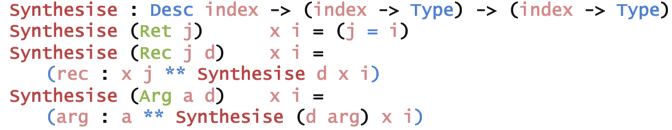
\includegraphics[scale=0.5]{Figures/SynthesisingData.png}
\end{center}
\caption{Synthesising Descriptions into Actual Types}
\label{fig:synthdata}
\end{figure}

We are able to synthesise our descriptions to actual types using \texttt{Synthesise}; However, an issue occurs when we want to use it since it requires the final form of the described datatype as input but the only way to synthesise the datatype is using \texttt{Synthesise} itself.
In order to ``tie the knot'' and complete input for \texttt{Synthesise}, we define a final datatype \texttt{Data} in the core theory which takes a description and provides the final form of the described datatype (see Figure~\ref{fig:datafromdesc}).
\texttt{Data} has only one constructor namely \texttt{Con} which takes as input the synthesised version of the description \texttt{d} with \texttt{Data d} serving as argument for the final form of the datatype in \texttt{Synthesise}. This works since each time we face a recursive argument it must be constructed using \texttt{Con} which avoids a infinite loop in \texttt{Synthesise} as long as the elements that are constructed are smaller in size; Luckily, the typesystem of Idris ensures \textit{totality} of functions and as such doesn't permit the creation of values that are infinitely sized except when the arguments are explicitly declared as such using the \texttt{Inf} type.

\begin{figure}[ht]
\begin{center}
    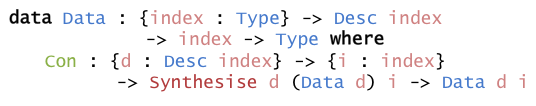
\includegraphics[scale=0.5]{Figures/TyingTheSynthesisKnot.png}
\end{center}
\caption{Knot-tying the Synthesised Description with Itself}
\label{fig:datafromdesc}
\end{figure}

\subsection{Example: Constructing Vectors}
\label{sub:Example:Constructing Vectors}

\begin{figure}[ht]
\begin{center}
    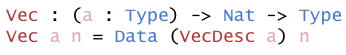
\includegraphics[scale=0.5]{Figures/VectorSynthesisedDesc.png}
\end{center}
\caption{Synthesised Version of Vector Description}
\label{fig:synthversvecdesc}
\end{figure}

\begin{figure}[ht]
\begin{center}
    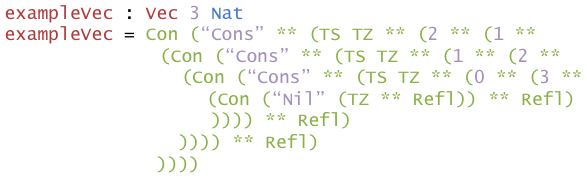
\includegraphics[scale=0.5]{Figures/VectorSynthesisedExample.png}
\end{center}
\caption{Example Vector representing ``[1,2,3]`` as a Value of a Synthesised Description}
\label{fig:exmvecsynthvecdesc}
\end{figure}

\begin{figure}[ht]
\begin{center}
    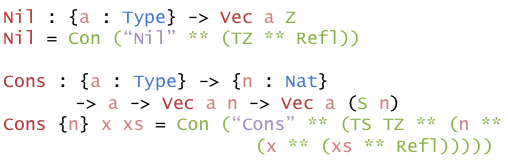
\includegraphics[scale=0.5]{Figures/VectorSynthesisedConstructors.png}
\end{center}
\caption{Functions for Constructing Values of Synthesised Vector Description}
\label{fig:funcconstrsynthvec}
\end{figure}

\begin{figure}[ht]
\begin{center}
    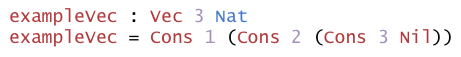
\includegraphics[scale=0.5]{Figures/VectorSynthesisedConstructorsExample.png}
\end{center}
\caption{More Readable Version of ``[1,2,3]`` using previously-defined Aliases}
\label{fig:exmvecsynthvecdescconstrs}
\end{figure}

\section{The (Mostly) Gentle Art of Levitation}
\label{sec:TheMostlyGentleArtofLevitation}
\textit{The elegance of a complete theorem for both ordinary and generic programming. Highlighting of possible issues with performance.}

\chapter{Partial Evaluation}
\label{cha:PartialEvaluation}

\section{Functions and Constant Inputs}
\label{sec:FunctionsandConstantInputs}
\textit{General introduction about partial evaluation.}

\section{Binding-time Analyses of Programs}
\label{sec:Binding-timeAnalysisofPrograms}
\textit{Finding the relevant constant parts of the program.}

\section{Specialisation as a Form of Optimization}
\label{sec:SpecialisationasaFormofOptimization}
\textit{Performance benefits of program specialisation. Pitfalls.}

\chapter{Levitating Idris}
\label{cha:LevitatingIdris}

\section{A Pragmatic Implementation of Levitation}
\label{sec:APragmaticImplementationofLevitation}
\textit{How the general concept of levitation was transferred to Idris.}

\section{Description Synthesis from Ordinary Data Declarations}
\label{sec:DescriptionSynthesisFromOrdinaryDataDeclarations}
\textit{How ordinary data-declarations are synthesized to levitational descriptions.}

\chapter{Practical Examples}
\label{cha:PracticalExamples}

\section{Generic Deriving}
\label{sec:GenericDeriving}
\textit{Examples of generic deriving of algorithms like decidable equality, pretty printing and possibly eliminators via generic structure.}

\section{Uniplate for Idris}
\label{sec:UniplateforIdris}
\textit{A version of the Uniplate library for Idris based on} \url{http://community.haskell.org/~ndm/uniplate/} \textit{and} \url{http://www-ps.informatik.uni-kiel.de/~sebf/projects/traversal.html} \textit{.
This is useful for traversing structures in a generic fashion and especially when dealing with small changes in large data structures (such as compiler ADTs)}

\chapter{Optimizing Idris for Flight}
\label{cha:OptimizingIdrisforFlight}

\section{Specialising Constructors for Specific Types}
\label{sec:SpecialisingConstructorsforSpecificTypes}
\textit{How generalized constructors of described types, are specialised as ordinary data structures.}

\section{Online Erasure of Unused Arguments}
\label{sec:OnlineErasureofUnusedArguments}
\textit{How some type infromation is to be erased at compile time to reduce elaboration overhead. Very hypothetical.}

\section{Static Initialization of Generic Functions}
\label{sec:StaticInitializationofGenericFunctions}
\textit{How algorithms that are dependent on the generic structure of a datatype are optimized. Discuss benefits of having a JIT/Profiling information for future work.}

\chapter{Evaluation}
\label{cha:Evaluation}

\chapter{Discussion}
\label{cha:Discussion}

\section{Future Work}
\label{sec:FutureWork}

\section{Conclusion}
\label{sec:Conclusion}

\appendix
\bibliography{report.bib}
\end{document}
